%BEGIN_FOLD
\documentclass[openany,twoside, notitlepage,letterpaper,11pt]{book}

%%% These are the packages that are used
%used for custom page headers and page numbering
\usepackage{fancyhdr}

%adds TeX fonts from the American Mathematical Society.
\usepackage{amsfonts}

%Sets the bounds of the page margins
\usepackage[top=1in, bottom=1in, left=0.7in, right=.7in]{geometry}

%Various useful packages
\usepackage{amsmath,amssymb, amscd,amsbsy, amsthm, enumerate}
\usepackage{mdframed, titlesec, setspace,verbatim, multicol, caption}
\usepackage[unicode]{hyperref}
\usepackage{wasysym}
\usepackage{tikz, polynom}
\usepackage{xcolor}
\usepackage{etoolbox}

%enables the ability of including pages from a pdf.
\usepackage{pdfpages}

%enables drawings of circuit diagrams
\usepackage{circuitikz}

%enables indexing
\usepackage{makeidx} 

%enables changing the bibliography name
\usepackage[nottoc,notlof,notlot]{tocbibind}

%makes the index size footnote
\usepackage[font=footnotesize, columns=3]{idxlayout}

%Adds extra symbols
\usepackage{mathrsfs, upgreek}

%Allows for tables with cells that span multiple rows and columns
\usepackage{multirow}

%Used for adding code chunks with proper formatting.
\usepackage{listings}

%This is where settings for the latex file are stored.
%%Version Number
\newcommand{\Version}{0.012}
%%Version

%%% Page formatting
%\setlength{\headsep}{30pt}
\setlength{\parindent}{25pt}
\setlength{\textheight}{9in}

%Rename the bibliography to References.
\renewcommand\bibname{References}


%%% Header and Footer Info
\pagestyle{fancy}
\fancyhead[LO]{\small {\textbf{Antonius' Handbook -- Volume II. Version \Version}}}
\fancyhead[RE]{\small {\textbf{Antonius' Handbook -- Volume II. Version \Version}}}
\fancyhead[C]{}
\fancyhead[RO]{\small \thepage}
\fancyhead[LE]{\small \thepage}
\fancyfoot[L]{}
\fancyfoot[C]{}
\fancyfoot[R]{}


\patchcmd{\chapter}{plain}{empty}{}{}
\titleformat{\chapter}[display]
{\normalfont\huge\bfseries}{}{0pt}{\Huge}
\titlespacing*{\chapter} {0pt}{-50pt}{10pt}

%re-defines the plain page style
\fancypagestyle{plain}{%
	\fancyhf{}
	\rhead{\thepage}
	\renewcommand{\headrulewidth}{0pt}}


%%Different lstlisting formats go here

\definecolor{backcolour}{rgb}{0.95,0.95,0.92}
\definecolor{commentcolour}{rgb}{.00,.245,.0}

\lstdefinestyle{sharpc}{language=[Sharp]C, tabsize=3, backgroundcolor=\color{backcolour},breaklines=true, basicstyle=\footnotesize, showstringspaces=false, commentstyle=\color{commentcolour}, keywordstyle=\color{blue}}

\lstdefinestyle{cpp}{language=C++, tabsize=3, backgroundcolor=\color{backcolour},breaklines=true, basicstyle=\footnotesize, showstringspaces=false, commentstyle=\color{commentcolour}, keywordstyle=\color{blue}}

\lstdefinestyle{bash}{language=Bash, tabsize=3, backgroundcolor=\color{backcolour},breaklines=true, basicstyle=\footnotesize, showstringspaces=false, commentstyle=\color{commentcolour}, keywordstyle=\color{blue}}

\lstdefinestyle{html}{language=html, tabsize=3, backgroundcolor=\color{backcolour},breaklines=true, basicstyle=\footnotesize, showstringspaces=false, commentstyle=\color{commentcolour}, keywordstyle=\color{blue}}

%This is where custom definitions and variables are defined and stored.
\newcommand{\andspace}[1]{\hspace{#1}\textrm{and}\hspace{#1}}

\numberwithin{equation}{section}
\setlength{\columnsep}{.5cm}
\setlength{\columnseprule}{1pt}
\def\columnseprulecolor{\color{black}}

\newcommand{\abs}[1]{\left| #1 \right|}
\newcommand{\inner}[1]{\langle #1 \rangle}
\newcommand{\norm}[1]{\left\lVert#1\right\rVert}
\newcommand{\spanvect}{\textnormal{span}}
\newcommand{\union}{\cup}
\newcommand{\Union}{\bigcup}

\newcommand\idx[1]{\textbf{#1}\index{#1}}

%create a section without making the section title.
\newcommand\invisiblesection[1]{%
	\refstepcounter{section}%
	\addcontentsline{toc}{section}{\protect\numberline{\thesection}#1}%
	\sectionmark{#1}}

%Makes a chapter with no title
\makeatletter
\newcommand{\unchapter}[1]{%
	\begingroup
	\let\@makechapterhead\@gobble % make \@makechapterhead do nothing
	\chapter{#1}
	\endgroup
}
\makeatother


%%% This defines the solution environment for you to write your solutions
\newenvironment{soln}
{\let\oldqedsymbol=\qedsymbol
	\renewcommand{\qedsymbol}{$ $}
	\begin{proof}[\bfseries\upshape \color{blue}Derivation]\color{blue}}
	{\end{proof}
	\renewcommand{\qedsymbol}{\oldqedsymbol}}

\newenvironment{note}
{\let\oldqedsymbol=\qedsymbol
	\renewcommand{\qedsymbol}{$ $}
	\begin{proof}[\bfseries\upshape \color{red}Note]\color{red}}
	{\end{proof}
	\renewcommand{\qedsymbol}{\oldqedsymbol}}


%theorem
\newcounter{theo}[section] \setcounter{theo}{0}
\renewcommand{\thetheo}{\arabic{section}.\arabic{theo}}
\newenvironment{theo}[2][]{%
	\refstepcounter{theo}%
	\ifstrempty{#1}%
	{\mdfsetup{%
			frametitle={%
				\tikz[baseline=(current bounding box.east),outer sep=0pt]
				\node[anchor=east,rectangle,fill=blue!20]
				{\strut Theorem~\thetheo};}}
	}%
	{\mdfsetup{%
			frametitle={%
				\tikz[baseline=(current bounding box.east),outer sep=0pt]
				\node[anchor=east,rectangle,fill=blue!20]
				{\strut Theorem~\thetheo:~#1};}}%
	}%
	\mdfsetup{innertopmargin=10pt,linecolor=blue!20,%
		linewidth=2pt,topline=true,%
		frametitleaboveskip=\dimexpr-\ht\strutbox\relax
	}
	\begin{mdframed}[]\relax%
		\label{#2}}{\end{mdframed}}
%%%%%%%%%%%%%%%%%%%%%%%%%%%%%%
%Lemma
\newcounter{lemm}[section] \setcounter{lemm}{0}
\renewcommand{\thelemm}{\arabic{chapter}.\arabic{lemm}}
\newenvironment{lemm}[2][]{%
	\refstepcounter{lemm}%
	\ifstrempty{#1}%
	{\mdfsetup{%
			frametitle={%
				\tikz[baseline=(current bounding box.east),outer sep=0pt]
				\node[anchor=east,rectangle,fill=green!20]
				{\strut Lemma~\thelem};}}
	}%
	{\mdfsetup{%
			frametitle={%
				\tikz[baseline=(current bounding box.east),outer sep=0pt]
				\node[anchor=east,rectangle,fill=green!20]
				{\strut Lemma~\thelem:~#1};}}%
	}%
	\mdfsetup{innertopmargin=10pt,linecolor=green!20,%
		linewidth=2pt,topline=true,%
		frametitleaboveskip=\dimexpr-\ht\strutbox\relax
	}
	\begin{mdframed}[]\relax%
		\label{#2}}{\end{mdframed}}
%%%%%%%%%%%%%%%%%%%%%%%%%%%%%%
%Proof
\newcounter{prf}[section]\setcounter{prf}{0}
\renewcommand{\theprf}{\arabic{chapter}.\arabic{prf}}
\newenvironment{prf}[2][]{%
	\refstepcounter{prf}%
	\ifstrempty{#1}%
	{\mdfsetup{%
			frametitle={%
				\tikz[baseline=(current bounding box.east),outer sep=0pt]
				\node[anchor=east,rectangle,fill=red!20]
				{\strut Proof~\theprf};}}
	}%
	{\mdfsetup{%
			frametitle={%
				\tikz[baseline=(current bounding box.east),outer sep=0pt]
				\node[anchor=east,rectangle,fill=red!20]
				{\strut Proof~\theprf:~#1};}}%
	}%
	\mdfsetup{innertopmargin=10pt,linecolor=red!20,%
		linewidth=2pt,topline=true,%
		frametitleaboveskip=\dimexpr-\ht\strutbox\relax
	}
	\begin{mdframed}[]\relax%
		\label{#2}}{\qed\end{mdframed}}
%%%%%%%%%%%%%%%%%%%%%%%%%%%%%%
%Definition
\newcounter{defn}[section] \setcounter{defn}{0}
\renewcommand{\thedefn}{\arabic{chapter}.\arabic{defn}}
\newenvironment{defn}[2][]{%
	\refstepcounter{defn}%
	\ifstrempty{#1}%
	{\mdfsetup{%
			frametitle={%
				\tikz[baseline=(current bounding box.east),outer sep=0pt]
				\node[anchor=east,rectangle,fill=gray!20]
				{\strut Definition~\thedefn};}}
	}%
	{\mdfsetup{%
			frametitle={%
				\tikz[baseline=(current bounding box.east),outer sep=0pt]
				\node[anchor=east,rectangle,fill=gray!20]
				{\strut Definition~\thedefn:~#1};}}%
	}%
	\mdfsetup{innertopmargin=10pt,linecolor=gray!20,%
		linewidth=2pt,topline=true,%
		frametitleaboveskip=\dimexpr-\ht\strutbox\relax
	}
	\begin{mdframed}[nobreak=true]\relax%
		\label{#2}}{\end{mdframed}}
%Fancy Box
\newcounter{fancybox}[section] \setcounter{fancybox}{0}
\renewcommand{\thefancybox}{\arabic{chapter}.\arabic{fancybox}}
\newenvironment{fancybox}[2][]{%
	\refstepcounter{fancybox}%
	\ifstrempty{#1}%
	{\mdfsetup{%
			frametitle={%
				\tikz[baseline=(current bounding box.east),outer sep=0pt]
				\node[anchor=east,rectangle,fill=orange!20]
				{\strut ~\thefancybox};}}
	}%
	{\mdfsetup{%
			frametitle={%
				\tikz[baseline=(current bounding box.east),outer sep=0pt]
				\node[anchor=east,rectangle,fill=orange!20]
				{\strut ~\thefancybox:~#1};}}%
	}%
	\mdfsetup{innertopmargin=10pt,linecolor=orange!20,%
		linewidth=2pt,topline=true,%
		frametitleaboveskip=\dimexpr-\ht\strutbox\relax
	}
	\begin{mdframed}[]\relax%
		\label{#2}}{\end{mdframed}}






% Define the questions environment
\newenvironment{questions}{%
	\begin{tcolorbox}[
		colback=orange!10,
		colframe=orange!50,
		arc=0pt,
		boxrule=1pt,
		title={\faQuestion\ Questions},
		fonttitle=\bfseries,
		coltitle=blue!50!black,
		colbacktitle=yellow!20,
		attach title to upper={\par},
		boxsep=0pt,
		]
		\begin{itemize}  % Start the itemize environment
			\BODY  % This will contain the list of questions
		\end{itemize}  % End the itemize environment
	\end{tcolorbox}
}

% define interesting note
\newenvironment{interestingnote}{
	\begin{tcolorbox}[
		colback=green!10,  % Very light green background color of the box
		colframe=green!50,  % Border color of the box
		arc=0pt,  % Adjust the corner radius of the box
		boxrule=1pt,  % Border thickness
		title={\faLightbulb\ Interesting Note},  % The lightbulb icon and title
		fonttitle=\bfseries,  % Font style for the title
		coltitle=blue!50!black,  % Color for the title text
		colbacktitle=yellow!20,  % Background color for the title
		attach title to upper={\par},
		boxsep=0pt,  % Adjust the space between the content and the box
		]
	}{
	\end{tcolorbox}
}

\definecolor{lightpurple}{RGB}{220,180,240}

\newenvironment{quotationbox}{
	\begin{tcolorbox}[
		colback=lightpurple!10,  % Very light purple background color of the box
		colframe=lightpurple!50,  % Border color of the box
		arc=0pt,  % Adjust the corner radius of the box
		boxrule=1pt,  % Border thickness
		title={\faQuoteLeft\ Quotation},  % The quotation icon and title
		fonttitle=\bfseries,  % Font style for the title
		coltitle=blue!50!black,  % Color for the title text
		colbacktitle=yellow!20,  % Background color for the title
		attach title to upper={\par},
		boxsep=0pt,  % Adjust the space between the content and the box
		]
	}{
	\end{tcolorbox}
}

% define a URL
\newenvironment{urlbox}{
	\begin{tcolorbox}[
		colback=blue!10,  % Very light green background color of the box
		colframe=blue!50,  % Border color of the box
		arc=0pt,  % Adjust the corner radius of the box
		boxrule=1pt,  % Border thickness
		title={URL},  % The lightbulb icon and title
		fonttitle=\bfseries,  % Font style for the title
		coltitle=blue!50!black,  % Color for the title text
		colbacktitle=yellow!20,  % Background color for the title
		attach title to upper={\par},
		boxsep=0pt,  % Adjust the space between the content and the box
		]
	}{
	\end{tcolorbox}
}

\newcommand{\unfinished}{%
	\par\noindent%
	\setlength{\fboxsep}{10pt} % Adjust the padding
	\fcolorbox{red}{red!20}{%
		\begin{minipage}{\dimexpr\linewidth-2\fboxsep}%
			\vspace{5pt} % Adjust the vertical spacing
			\centering
			\textcolor{red}{\textbf{\faExclamation\ Section in Progress\ \faExclamation}}
			\vspace{5pt} % Adjust the vertical spacing
		\end{minipage}%
	}%
	\par
}

%creates the title page
\title{
\includegraphics[scale=.22]{./Images/Covers/AH3.png}
	\\ \vspace{1.5cm} Useful Formulas, Constants, Units and Definitions \\ Volume II - Programmers Paradise \\ Version \Version}
\date{}
\author{Compiled by: Antonius William Torode\\ Natural Science Department: Michigan State University \\ Written in: \LaTeX}

\makeindex
%\addcontentsline{toc}{chapter}{Index}
%END_FOLD

%%% Document Starts now
\begin{document}

%Begin the front matter.
\frontmatter
%Begins title page.
\maketitle
\thispagestyle{empty}
\pagestyle{empty}
\begin{center}
	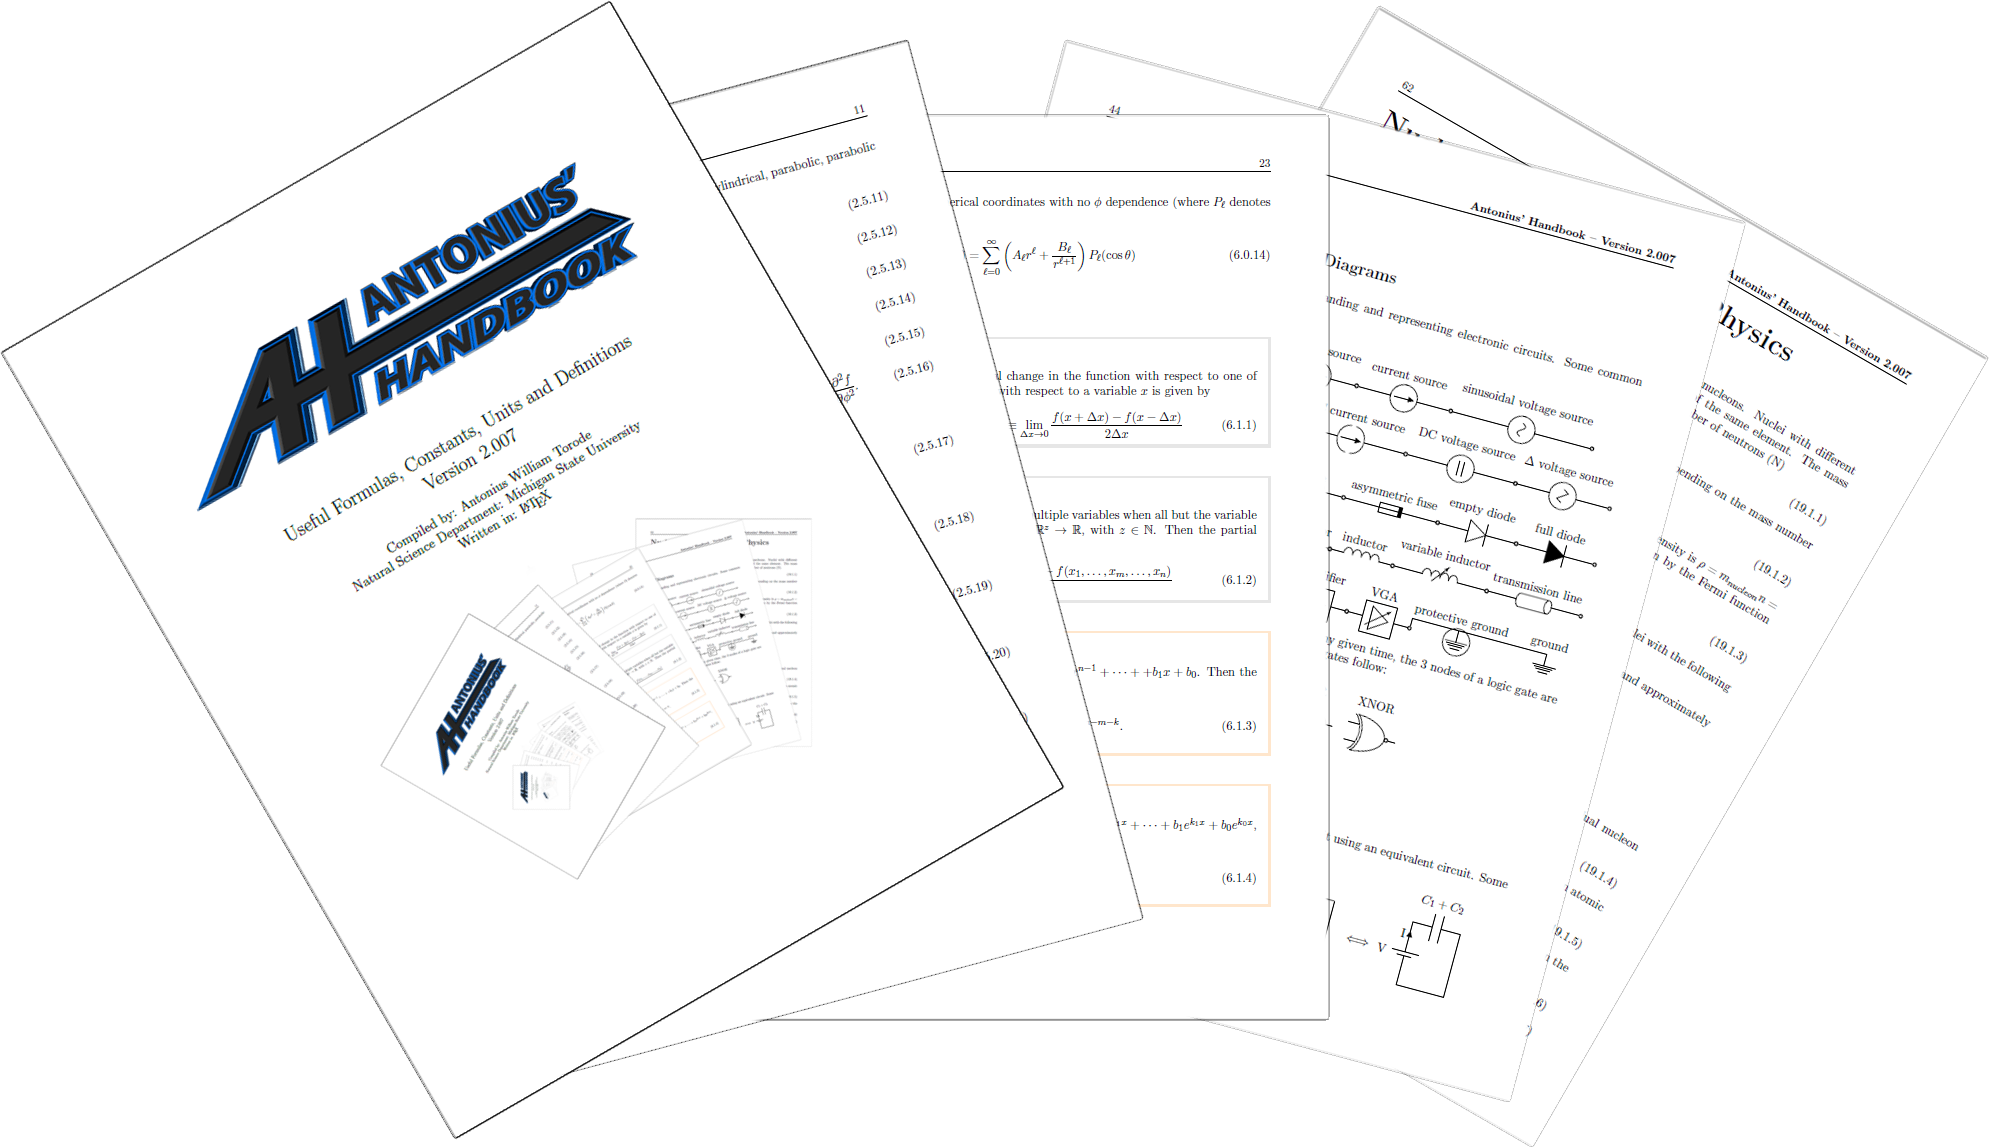
\includegraphics[scale=1.8]{./Images/Covers/background_tunnel.png}
\end{center}

%Copywrite page
\pagestyle{empty}
%% copyrightpage
\begingroup
\footnotesize
\parindent 0pt
\parskip \baselineskip
\textcopyright{} 2016 Antonius Torode \\
All rights reserved.

This work may be distributed and/or modified under the conditions of Antonius’ General Purpose License (AGPL).

The original maintainer of this work is: Antonius Torode.

The current maintainer of this work is: Antonius Torode.

Published by Antonius Torode. 

Hosted at: https://torodean.github.io/AHandbook.html

Github Repository: https://github.com/torodean/Antonius-Handbook-II

\begin{center}
\begin{tabular}{ll}
First Personal Release (Version 0.000): & June 2017 \\
First Public Release (Version 1.000): &  N/A \\
Most Current Revision Date (Version \Version): & \today 
\end{tabular}
\end{center}

\vfill

Torode, A.\\
\hspace*{1em} Antonius' Handbook. \\
\hspace*{2em} Michigan State University -- \\
\hspace*{2em} Department of Physics \& Astronomy. \\
\hspace*{2em} 2016, Graduate. \\
\hspace*{2em} Volume II. \\
\hspace*{2em} Version: \Version



\endgroup
\clearpage

%Preface page
\begin{center}
	\textbf{Preface}
\end{center}

This document is a compilation of useful programming formulations, definitions, constants, and general information used throughout my own schooling and research as a reference while furthering education. It's purpose is to provide a complete 'encyclopedia' per say of various codes, syntax and significant ideas used often. The idea and motivation behind it is to be a quick reference providing easily accessible access to necessary information for either double checking or recalling proper formulations or algorithms for use in various situations due to my own shortcomings in matters of memorization. All the material in this document was either directly copied from one of the references listed at the end or derived from scratch. On occasion typos may exist due to human error but will be corrected when discovered.
	
The version number is updated every time the document is modified. This ensures that there is no two copies with different information and identical version numbers. The latest update date is automatically set to the current date each time the document is edited. Please refrain from distributing this handbook without permission from the original author/compiler. This book is formatted for printing.

For more information about this book or details about how to obtain your own copy please visit:
\begin{center}
	https://torodean.github.io/AHandbook.html
\end{center}
\begin{center}
	\textbf{Disclaimer}
\end{center}

This book contains codes, formulas, definitions, and theorems that by nature are very precise. Due to this, some of the material in this book was taken directly from other sources. This is only such in cases where a change in wording or codes could cause ambiguities or loss of information quality.  Following this, all known sources used are listed in the references section.

%Begins blank page.
\thispagestyle{empty}
\newpage
\vspace*{\stretch{1}}
\begin{center}
	\textit{This page intentionally left blank.\\ (Yes, this is a contradiction.)}
\end{center}
\vspace*{\stretch{1}}

%Begins table of contents
\tableofcontents


%Begin the mainmatter.
\setlength{\parindent}{0pt}
\mainmatter
\pagestyle{fancy}
\chapter{Introduction}
\thispagestyle{fancy}

This document is still under the initial formatting stages and useful information will be added soon. When it has sufficient information to be ready for distribution the version will be updated to 1.000.

\newpage
\chapter{Linux}
\thispagestyle{fancy}
\lstset{language=Bash, style=terminalstyle}

Linux is a broad subcategory that encompass a large family of free and open sourced operating systems. Installing, setting up, and using a Linux based operating system is the perfect way for anyone to gain knowledge, understanding, and practice of how a computer system truly works. Unlike the end user experience with Windows and Mac OS, Linux has a much higher capability for customization and a higher degree of freedom. With that said, Linux is not necessarily more user friendly to the new or average computer user, however it is free in most cases!








\section{System Related Commands\index{System Related Commands}}

Retrieve information and valid arguments for a command. This works with many commands.
\begin{lstlisting}
COMMAND --help   # COMMAND must be a valid command such as cd, ls, etc...
\end{lstlisting}

To view the \idx{history} of commands entered or \idx{delete} a history entry, you can use the \idx{history} command. This could be useful if you accidentally typed in your \idx{password} or something similar into the terminal.
\begin{lstlisting}
history               # View command history.
history -d <ID>       # Delete the history entry listed with number <ID>
\end{lstlisting}

Installing and updating packages using package managers such as \idx{apt}, \idx{yum}, or \idx{dnf}.
\begin{lstlisting}
sudo apt update  # Updates the list of available packages (APT)
sudo apt upgrade # Upgrades installed packages to their latest versions (APT)
sudo yum update  # Updates the list of available packages (Yum)
sudo yum upgrade # Upgrades installed packages to their latest versions (Yum)
sudo dnf update  # Updates the list of available packages (DNF)
sudo dnf upgrade # Upgrades installed packages to their latest versions (DNF)
\end{lstlisting}

Monitoring system resource usage using tools like \idx{top}, \idx{htop}, and \idx{iotop}.
\begin{lstlisting}
top   # Displays dynamic real-time information about running processes
htop  # An interactive process viewer
iotop # Displays I/O usage by processes in real-time
\end{lstlisting}

\idx{Changing directory} via terminal via the \idx{cd}command.
\begin{lstlisting}
cd /directory # Changes the directory to the subdirectory /directory
cd ..         # Goes back one directory
\end{lstlisting}

Getting \idx{current directory} via terminal
\begin{lstlisting}
pwd
\end{lstlisting}

How to display the processes that are currently running.
\begin{lstlisting}
ps aux
\end{lstlisting}

To search the results of a command for a string of characters one can use the grep command. For example:
\begin{lstlisting}
ps aux | grep "firefox"
\end{lstlisting}

Restore power/battery icon if it disappears on a laptop.
\begin{lstlisting}
/usr/lib/x86_64-linux-gnu/indicator-power/indicator-power-service &disown 
\end{lstlisting}

Restore volume icon/control button if it disappears.
\begin{lstlisting}
gsettings set com.canonical.indicator.sound visible true
\end{lstlisting}

Reset wifi services in case the connection gets lost.
\begin{lstlisting}
sudo systemctl restart network-manager.service
\end{lstlisting}

Turn off LCD display.
\begin{lstlisting}
xset dpms force off  // Turns off display.
\end{lstlisting}

Change or view the host name of a computer with the hostname file.
\begin{lstlisting}
sudo nano /etc/hostname # Opens this file using nano for editing.
hostname                # Command to see what the current hostname is.
\end{lstlisting}







\section{Remote Connections (SSH)\index{Remote Connections}\index{SSH}}


Accessing remote systems using \idx{Secure Shell} (\idx{SSH}).
\begin{lstlisting}
ssh username@hostname     # Connects to the remote system using SSH
\end{lstlisting}

Transferring files securely between systems using \idx{scp} or \idx{sftp}.
\begin{lstlisting}
# Copies a file from local to remote system
scp /path/to/local/file username@hostname:/path/to/remote/location

# Copies a file from remote to local system
scp username@hostname:/path/to/remote/file /path/to/local/location

# Initiates interactive SFTP session with remote system
sftp username@hostname    
\end{lstlisting}

Accessing remote desktops using \idx{X11 forwarding} and X terminal.
\begin{lstlisting}'
# Enables X11 forwarding for remote system
ssh -X username@hostname

# Opens a new X terminal window from remote system
xterm        
\end{lstlisting}

Securely transferring files between systems using \idx{rsync}.
\begin{lstlisting}
# Synchronizes files and directories between local and remote systems
rsync -avz /source/path username@hostname:/destination/path
\end{lstlisting}

Accessing remote systems via graphical interface using tools like \idx{VNC} or \idx{XRDP}.
\begin{lstlisting}
# Opens a VNC session to remote system
vncviewer hostname

# Opens a Remote Desktop Protocol (RDP) session to remote system
rdesktop hostname
\end{lstlisting}

Establishing persistent remote connections using tools like \idx{tmux} or \idx{screen}.
\begin{lstlisting}
tmux new -s sessionname    # Creates a new tmux session
screen -S sessionname      # Creates a new screen session
\end{lstlisting}








\section{Files and Storage}

To find a file within a folder or its sub-folders, you can use the \idx{find}\index{find} command.
\begin{lstlisting}
find -name "fileName.txt"  # Finds a file named fileName.txt
find -name "file*"  # Finds a file containing "file" in its name.
\end{lstlisting}

Copy a file or directory to a different computer
\begin{lstlisting}
# To copy a file.
scp -v <File Path> username@computer:"<path to copy to>"

# To copy a directory.
scp -rv <File Path> username@computer:"<path to copy to>"
\end{lstlisting}

Show information about the file system on which each FILE resides, or all file systems by default.
\begin{lstlisting}
df 
\end{lstlisting}

Retrieve the Disk Usage (file sizes) of a directory or its contents.
\begin{lstlisting}
du        # List the size of the subdirectories.
du -sh    # List the size of the directory in a human readable format.
du -ah    # Lists the size of all files in the directory.
\end{lstlisting}

List information about File(s) (in the current directory by default). You can specify the number of entries you want listed using the \idx{head} and \idx{tail} commands.
\begin{lstlisting}
ls         # list all items in a directory
ls -1      # list all items in a directory (one item per line)
ls -lh     # list all items with size, owner, and date modified
ls -lu     # list all items with size, owner, and date accessed.
ls -lc     # list all items with size, owner, and date of status change. 
ls -lhrt   # Useful ls output

ls -lhrt | head -4	 # Outputs only the first four entires
ls -lhrt | tail -4	 # Outputs only the last four entires
\end{lstlisting}

The \idx{stat} command is used to display detailed information about a file or directory. It provides various details such as file type, permissions, size, timestamps (access, modify, and change), and more.
\begin{lstlisting}
stat filename
\end{lstlisting}

To list all of the \idx{block devices} (and hence \idx{partitions}) detected by the machine, you can use the `\idx{lsblk}' command. Block devices are physical or \idx{virtual} devices that can be used for data storage, such as hard drives, SSDs, and partitions.\begin{lstlisting}
lsblk
\end{lstlisting}

To \idx{mount} and \idx{unmount} a partition
\begin{lstlisting}
sudo mount <DEVICE TO MOUNT> <MOUNT POINT>
sudo mount /dev/sdb1/ /mnt/       # example of mounting
sudo umount <DEVICE TO MOUNT> <MOUNT POINT>
sudo umount /dev/sdb1/ /mnt/      # example of mounting
\end{lstlisting}


To open a \idx{pdf} via terminal, most generic desktop environments support
\begin{lstlisting}
xdg-open filename.pdf
\end{lstlisting}

Creating backups using tools like \idx{tar}, \idx{rsync}, or \idx{backuppc}.
\begin{lstlisting}
# Creates a compressed tarball of a directory
tar -czvf backup.tar.gz /path/to/directory

# Synchronizes files and directories between two locations
rsync -avz /source/path /destination/path
\end{lstlisting}











\section{Users and Groups}

List all users
\begin{lstlisting}
cut -d: -f1 /etc/passwd
\end{lstlisting}

Create a new user using the \idx{useradd} command.
\begin{lstlisting}
sudo useradd [options] <USERNAME>      # Creates a user.
sudo useradd -e 2016-02-05 <NAME>      # Creates a user that expites on a day.
sudo useradd <USERNAME> -G <GROUPNAME> # Adds a user to a group upon creation.
useradd --help                         # See full useradd options.
\end{lstlisting}

Change a users password using passwd.
\begin{lstlisting}
passwd <USERNAME>
\end{lstlisting}

Change the user in terminal using the \idx{su} command.
\begin{lstlisting}
su - <USERNAME>
\end{lstlisting}

Add a user to the sudoers group
\begin{lstlisting}
usermod -aG sudo <USERNAME>
\end{lstlisting}

Managing user permissions and file ownership using \idx{chmod}, \idx{chown}, and \idx{chgrp}.
\begin{lstlisting}
chmod 755 file         # Changes file permissions to read, write, and execute for owner, and read and execute for group and others.
chmod a+x file         # Changes file permissions to include execute permissions.
chown user:group file  # Changes the owner and group of the file.
chgrp group file       # Changes the group of the file.
\end{lstlisting}












\section{Networking\index{Networking}}

The \idx{ifconfig} command is for viewing IP configuration information and configuring network interface parameters.
\begin{lstlisting}
ifconfig
\end{lstlisting}

The \idx{traceroute} command is for printing the route that packets take to a network host.
\begin{lstlisting}
traceroute
\end{lstlisting}

The \idx{Domain Information Groper} is used to perform DNS lookups and display answers returned from the DNS servers.
\begin{lstlisting}
dig
\end{lstlisting}

The \idx{telnet} command connects the destination host:port via the telnet protocal. An established connection means connectivity between two hosts is properly working.
\begin{lstlisting}
telnet
\end{lstlisting}

The \idx{nslookup} command is for querying Internet domain name servers.
\begin{lstlisting}
nslookup
\end{lstlisting}

The \idx{netstat} command is used to review open network connections and open sockets. 
\begin{lstlisting}
netstat
\end{lstlisting}

The \idx{nmap} command is used to check for opened ports on a server
\begin{lstlisting}
nmap <SERVER NAME>
\end{lstlisting}

The \idx{ifup} and \idx{ifdown} commands are used to disable network interfaces.
\begin{lstlisting}
# Enables an ethernet parameter
ifup <ETHERNET INTERFACE PARAMETER>
ifup eth0  # example: enables 'eth0'

# Disables an ethernet parameter
ifdown <ETHERNET INTERFACE PARAMETER>
ifdown eth0  # example: disables 'eth0'
\end{lstlisting}

Enable/Disable \idx{IPv6}. This is only a temporary solution as it may turn itself back on after some time.
\begin{lstlisting}
# Use these two commands to disable IPv6
sudo sysctl -w net.ipv6.conf.all.disable_ipv6=1
sudo sysctl -w net.ipv6.conf.default.disable_ipv6=1

# Use these two commands to re-enable IPv6
sudo sysctl -w net.ipv6.conf.all.disable_ipv6=0
sudo sysctl -w net.ipv6.conf.default.disable_ipv6=0
\end{lstlisting}







\subsection{Redirecting program output}

When outputting to a file, there is an append and an overwrite operator.
\begin{lstlisting}
command > output.txt    // Writes output to output.txt
command >> output.txt   // Appends output to output.txt
\end{lstlisting}
To redirect all output from a program (including \idx{stdout} and \idx{stderr}), you can use 
\begin{lstlisting}
command -args > output.txt 2>&1
\end{lstlisting}






\section{Shell/Bash Scripting\index{Bash}}

\lstset{language=Bash, style=shellstyle}

To create a shell script you must create a new text file and save it as a '.sh' file. The file should start with the directory to the proper shell which is generally the default below. The first line (starting with a \idx{shebang} '\#!') is not a comment, but instead is treated by Unix as "which shell do I use to run this code." In our case, the Bourne shell will be used \cite{linux: shell scripting}. Furthermore, to create a shell application that has parameters, with a help screen to explain those parameters, you can apply the following template.
\begin{lstlisting}
#!/bin/sh
# This is a comment!

# This creates a method to print the usage of the script
usage()
{
	cat << EOF
purpose: This explains the purpose of the script
Usage:   $0 [opts]

OPTIONS:
	-h         Display this help message
	-f <file>  File to input
	-v         Boolean-type flag as parameter
	
EOF


# This parses the arguments input to the script. The ":" specifies a parameter is expected with the input flag.
while getopts "hf:v" OPTION; do
	case $OPTION in
		h)	usage			# Calls out usage method.
			exit 0			# Exits with error code 1 => success.
			;;				# Ends the specified case
		f)	fileInput=$OPTARG
			;;
		v)	verboseMode=1	# Sets verboseMode to true.
			;;
		*)	echo "Invalid option entered: -$OPTARG" >&2
			usage
			exit 2			# Exits with error code 2 => fail.
			;;
	esac					# completes out case statement
done

# This checks if a flag was used.
if [[ $verboseMode ]]; then
	echo "Verbose mode is activated!"
elif [[ ! $verboseMode ]]; then
	echo "Verbose mode is disabled!"
fi
}
\end{lstlisting}

To print text one can use the \idx{echo} command as follows.
\begin{lstlisting}
#!/bin/sh
echo Hello World
echo "Hello World"
echo -e "In order to print newline characters, use the e option!\n"
\end{lstlisting}

To make a file executable, or change the permissions in general the \idx{chmod} command can be used and is typically used as follows.
\begin{lstlisting}
chmod a+x <SCRIPTNAME>.sh					 # Make a script executable.
chmod -R 775 filesToChangePermissionsOf.ext  # Change the permissions of some file.
\end{lstlisting}

To modify the ownership of files you can specify the owner and group of a file(s) using \idx{chown}
\begin{lstlisting}
chown username:group file.txt   # Change the owner and group of a file.
chown -R :group folder          # Change only the group of some folder and its sub-folders.         
\end{lstlisting}

Shell script \idx{variables} are created by use of the equal sign. spaces in lines containing variables need to be avoided. To reference a variable, the '\$' character is used. Quotations are used to avoid ambiguities with spaces.
\begin{lstlisting}
#!/bin/sh
MY_VARIABLE="Hello World"    # Creates a variable.
echo $MY_VARIABLE            # Prints the variable.
\end{lstlisting}

To use a variable within a terminal session, you can use \idx{export} it to store it for that session.
\begin{lstlisting}
export PATH="$PATH:/home/user/.local/bin/" # Appends the PATH variable with a string
\end{lstlisting}

The \idx{touch} command can be used to create a new empty file.
\begin{lstlisting}
#!/bin/sh
echo "What is your name?"
read USER_NAME
echo "Hello $USER_NAME"
echo "I will create you a file called ${USER_NAME}_file"

# The quotations prevent multiple files from being called to touch.
touch "${USER_NAME}_file"
\end{lstlisting}

To determine the total number of files of a given file patter, you can use the \idx{wc} command to count the output of an ls command. To save the output of a script or command, you must enclose it within the correct elements of `\$()' such as below.
\begin{lstlisting}
totalFiles=$(ls -l $filePattern 2> /dev/null | wc -l)
\end{lstlisting}

To perform \idx{arithmetic} within shell scripts, you must use double parenthesis.
\begin{lstlisting}
firstVar=4
secondVar=7
addedVar=$(($firstVar+$secondVar))
\end{lstlisting}

To create a \idx{for loop} in shell, you can do so like the following:
\begin{lstlisting}
i=1
for file in $filePattern; do
	[[ ! -e $file ]] && continue
	echo "I see file number $i: $file"
	((i++))
done
\end{lstlisting}

Bash provides a feature called "\idx{brace expansion}," which allows you to generate arbitrary strings based on patterns using curly braces {}. While this feature is commonly used to generate sequences of numbers or letters, it can also be used in conjunction with command-line shortcuts to save time and improve efficiency.
\begin{lstlisting}
# This will create directory1, directory2, ... and directory5.
mkdir directory{1..5}
\end{lstlisting}




\section{Other}
\lstset{language=Bash, style=terminalstyle}

The \idx{mkfifo} command is used to create a new named pipe. A pipe is used to store the output of one program to be used in another.
\begin{lstlisting}
mkfifo namedPipe   # Creates a pip named "namedPipe".
ls > namedPipe     # Feeds the output of ls into namedPipe.
cat < namedPipe    # Feeds namedPipe into cat and displays the data from ls.
mkfifo namedPipe2 -m700  # Modifies the permissions of a created pipe.
\end{lstlisting}

\subsection{emacs}
\idx{Emacs} is a powerful text editor. You can open a document through emacs using the following. The ``-nw" flag indicates no GUI window should open (open in terminal).
\begin{lstlisting}
emacs doc.txt -nw
\end{lstlisting}
To toggle \idx{read-only mode} use C-x C-q.


%\newpage
%\chapter{Windows}
\thispagestyle{fancy}
\lstset{language=Bash, style=bash}

\begin{fancybox}[Windows Key Combinations]{}	
	Windows has various key combinations. These are used to do different things. For the purposes of this chart, the windows key will be represented by $\boxplus$.
	\begin{center}
		\begin{tabular}{l|l}
			Key combination & Descriptions \\
			\hline
			$\boxplus$ + R & Opens a run window. \\
			$\boxplus$ + m & Minimize all open windows. \\
			$\boxplus$ + E & Opens the explorer window. \\
			$\boxplus$ + UP & Minimize the currently opened window. \\
			$\boxplus$ + F & Opens search for searching files and folders. \\
			Alt + Tab & Change between open windows. \\
			CTRL + ALT + Delete & Provides user options such as changing password. \\
			CTRL + SHIFT + ESC & Opens Windows Task Manager. 
		\end{tabular}
	\end{center}
\end{fancybox}

To access the Windows 7 "God Mode" which is essentially a collection of administrator and troubleshooting features, create a folder with the following name:
\begin{lstlisting}
GodMode.{ED7BA470-8E54-465E-825C-99712043E01C}
\end{lstlisting}

To view system information, including RAM installed, graphics processor and more, run the following command
\begin{lstlisting}
dxdiag
\end{lstlisting} 

To view and manage the \idx{services} that are running on a machine, you can access the services.msc application by opening a run window and entering 
\begin{lstlisting}
services.msc	# Opens the services running.
\end{lstlisting}

To view and modify mouse settings, such as sensitivity or speed, you can open a run window and enter
\begin{lstlisting}
main.cpl		# Opens the mouse settings.
\end{lstlisting}

\newpage
\chapter{Mac}
\thispagestyle{fancy}
\lstset{}\lstset{language=Bash, style=shellstyle}

MacOS is Apple's proprietary Unix-based operating system tailored for Macintosh computers. It boasts a sleek graphical user interface (GUI) atop a Unix-like foundation, offering stability and security. Its software ecosystem encompasses a broad array of third-party applications accessible through the Mac App Store and other channels.

Notable features include seamless integration with Apple's ecosystem, such as iCloud and iOS devices, robust security measures like Gatekeeper and FileVault for app and disk encryption, respectively, and advanced privacy controls. MacOS also provides essential productivity tools and development support, including Xcode and Terminal, making it an appealing platform for software engineers and developers.


\begin{fancybox}[Mac Startup Options]{}	
	Mac has various startup features. To use them, hold the following keys down simultaneously upon startup as soon as you hear the startup chime:
	\begin{center}
		\begin{tabular}{l|l}
			Startup Keys & Descriptions \\
			\hline
			Command, R & Boot into OS X Recovery mode. \\
			C & Boot to external device such as CD, DVD, or USB. \\
			N & Netboot. \\
			Shift & Safe Boot. \\
			Command, V & Boot using verbose mode for comprehensive boot details. \\
			Command, S & Single user mode. \\
			Command, Option, P, R & Resetting the PRAM during boot. \\
			T & Enable target disk mode.
		\end{tabular}
	\end{center}
\end{fancybox}





%\newpage
%\chapter{C}
\thispagestyle{fancy}

\newpage
\chapter{C++}
\thispagestyle{fancy}
\lstset{language=C++, style=cpp}

\section{Basic Input and Output\index{Input and Output}}
To output text via a terminal you can use:
\begin{lstlisting}
std::string text = "Hello World!";
std::cout << text << std::endl; //std::endl is equivalent to the new-line character.
\end{lstlisting}

To get input as a user in the type of a std::string, you can use:
\begin{lstlisting}
std::string input = "";
std::cout << "Enter some text: ";
std::getline(std::cin, input);
\end{lstlisting}

\subsection{Simulate Key Strokes (Windows Only)\index{Simulate Key Strokes}}

First the correct files must be included and an event must be setup.
\begin{lstlisting}
#define WINVER 0x0500
#include <windows.h> 

INPUT ip;

ip.type = INPUT_KEYBOARD; // Set up a generic keyboard event.    
ip.ki.wScan = 0; // hardware scan code for key                                   
ip.ki.time = 0;
ip.ki.dwExtraInfo = 0;
\end{lstlisting}

After this, functions can be setup to simulate various keys based on the specific key codes, two examples of such are
\begin{lstlisting}
void space(){ 
	// Press the "space" key.  
	ip.ki.wVk = VK_SPACE; // virtual-key code for the "space" key.                                                                                
	ip.ki.dwFlags = 0; // 0 for key press                                                                                                        
	SendInput(1, &ip, sizeof(INPUT));
	
	// Release the "space" key                                                                                                                   
	ip.ki.wVk = VK_SPACE; // virtual-key code for the "space" key.                                                                                
	ip.ki.dwFlags = KEYEVENTF_KEYUP; // KEYEVENTF_KEYUP for key release                                                                          
	SendInput(1, &ip, sizeof(INPUT));
	Sleep(50);
}

void one(){ 
	// Press the "1" key.    
	ip.ki.wVk = 0x31; // virtual-key code for the "1" key.                                          
	ip.ki.dwFlags = 0; // 0 for key press                                                                                                        
	SendInput(1, &ip, sizeof(INPUT));
	
	// Release the "1" key.                                                                                                                    
	ip.ki.wVk = 0x31; // virtual-key code for the "1" key.                                                                                      
	ip.ki.dwFlags = KEYEVENTF_KEYUP; // KEYEVENTF_KEYUP for key release.                                                                          
	SendInput(1, \&ip, sizeof(INPUT));
	Sleep(50);
}
\end{lstlisting}

A similar method can be used to simulate mouse clicks. And example for left click follows
\begin{lstlisting}
void leftclick(){
	INPUT ip={0};
	// left down                                                                                                                                   
	ip.type = INPUT_MOUSE;
	ip.mi.dwFlags = MOUSEEVENTF_LEFTDOWN;
	SendInput(1,&Input,sizeof(INPUT));
	
	// left up                                                                                                                                     
	ZeroMemory(&Input,sizeof(INPUT));
	ip.type = INPUT_MOUSE;
	ip.mi.dwFlags = MOUSEEVENTF_LEFTUP;
	SendInput(1,&Input,sizeof(INPUT));
	Sleep(50);
}
\end{lstlisting}












\section{Variable Types\index{Variable Types}}

Creating and using a vector\index{Vector}.
\begin{lstlisting}
#include <vector>

int size1 = 5;
int size2 = 6;

//Creates a vector named V1 containing int's with a size of 5 and sets each element to 0. 
std::vector<int> V1(size1, 0); 

//Creates a 2-D vector (vector containing vectors) of size 5x6 named V2 containing doubles;
std::vector< std::vector<double>> V2(size1, std::vector<double>(size2, 0)); 

V1[0] = 8; //Sets the first element in V1 to 8.

V2[0][3] = 3.1415; //Sets the 4th element in the first row of V2 to 3.1415.

\end{lstlisting}













\subsection{Converting Between Types\index{Converting Between Types}}

\subsection*{std::string to int\index{std::string to int}}
To convert a string to an integer you can use the \textbf{stoi}\index{stoi} function:
\begin{lstlisting}
std::string text = "31415";
int number = std::stoi(text);
\end{lstlisting}

\subsection*{std::string to double\index{std::string to int}}
To convert a string to a double you can use the \textbf{stod}\index{stod} function:
\begin{lstlisting}
std::string text = "3.1415";
double number = std::stof(text);
\end{lstlisting}

















\section{Mathematical Commands}

\subsection*{Prime Number\index{Prime Number}}
A simple brute for method to determines if a number of type long is prime or not.
\begin{lstlisting}
bool isPrime(long num) {  
	int c = 0;   //c is a counter for how many numbers can divide evenly into num
	if (num == 0 || num == 1 || num == 4) {
		return false;
	}
	for (long i = 1; i <= ((num + 1) / 2); i++) {
		if (c < 2) {
			if (num % i == 0) {
				c++;
			}
		} else {
			return false;
		}
	}
	return true;
}
\end{lstlisting}















\section{System Commands\index{System Commands}}

\subsection*{Sleep\index{Sleep}}
Make the thread sleep for some amount of time using the std::chrono to determine the duration \cite{cpp:chrono}.
\begin{lstlisting}
#include <thread>
#include <chrono>

std::this_thread::sleep_for(std::chrono::milliseconds(50)); //Makes the system sleep for 50 milliseconds.

std::this_thread::sleep_for(std::chrono::seconds(50)); //Makes the system sleep for 50 seconds.
\end{lstlisting}

On a Windows specific program this can be simplified by including the windows.h header
\begin{lstlisting}
#include <windows.h>

Sleep(50); //Makes the system sleep for 50 milliseconds.

Sleep(5000); //Makes the system sleep for 50 seconds.
\end{lstlisting}












%\section{Qt Specific}




\newpage
\chapter{ROOT}
\thispagestyle{fancy}

Formatting a TString can be simplified by use of the Form function.

\begin{lstlisting}
const char *someText = "Hello World!";
int someInt = 2314;

//%s corresponts to a const char*
//%d corresponds to an integer
TString output = Form("I want to say %s a total of %d times", someText, someInt);

//This will output "I want to say Hello World! a total of 2314 times"
std::cout << output;
\end{lstlisting}

%\newpage
%\chapter{C\#\index{C\#}}
\thispagestyle{fancy}
\lstset{}\lstset{language=[Sharp]C, style=csharpstyle}

C\# is a powerful, object-oriented programming language developed by Microsoft as part of the .NET initiative in the early 2000s. Designed for building robust, scalable applications, C\# combines the productivity of modern, high-level languages with the performance and control of low-level languages. With its elegant syntax, rich standard library, and seamless integration with the .NET framework, C\# enables developers to create a wide range of applications, from web and desktop applications to mobile and gaming platforms. Key features of C\# include automatic memory management, type safety, and support for modern programming paradigms such as asynchronous programming and LINQ (Language-Integrated Query). Backed by a vibrant developer community and extensive documentation, C\# continues to be a popular choice for building enterprise-grade software solutions across various industries.

\myindent The language C\# is very similar to C++ and Java. All programming snippets listed in this section were tested and from a program created in Visual Studio 2013. Many of the functions written in this section depend on the Windows .Net application framework and may not function without that.

\section{Useful Application Functions}

Exit a program.
\begin{lstlisting}
//These are needed at the beginning of the file.
using System;
using System.Windows.Forms;

//This exits the program
public static void exitLOLA(){
	if (System.Windows.Forms.Application.MessageLoop){
		System.Windows.Forms.Application.Exit();     // WinForms app
	} else {
		System.Environment.Exit(1);     // Console app
	}
}
\end{lstlisting} 

The following will return the current Epoch time in seconds. This is useful for version control, random number generation, and more. Also, a demonstration of how ot set the current date as a string.
\begin{lstlisting}
//Sets the current date as a string.
private static string today = System.DateTime.Today.ToString("d");

//Returns the current epoch time in seconds (time passed since January 1, 1970).
public static long getEpochTime(){
	var epoch = (DateTime.UtcNow - new DateTime(1970, 1, 1, 0, 0, 0, DateTimeKind.Utc)).TotalSeconds;
	return (long)epoch;
}
\end{lstlisting}

The following can be used to increase the size of a terminal window for a terminal application make in Visual Studio.
\begin{lstlisting}
//Doubles the length of the output terminal window if the resolution on the computer permits it.
//Otherwise leaves it as the default.
public static void setScreenSize_double(){
	//determines the screen resolution to then determine the size of the output window.
	int origWidth = Console.WindowWidth;
	int origHeight = Console.WindowHeight;
	int height;
	int screenHeight = Screen.PrimaryScreen.Bounds.Height;
	
	if (screenHeight < 1080){
		height = origHeight;
	} else {
	height = origHeight * 2;
	}
	
	//int height = origHeight;
	Console.SetWindowSize(origWidth, height);       
}
\end{lstlisting}

Get the directory path that the executable file is located in.
\begin{lstlisting}
//returns the path that the program executable file is in.
public static string getProgramPath(){
	string path = System.IO.Path.GetDirectoryName(Assembly.GetEntryAssembly().Location);
	return path;
}
\end{lstlisting}










\section{Getting Windows System Information}

Return the system name
\begin{lstlisting}
//Returns the user defined system name.
public static string getSystemName() {
	systemName = Environment.MachineName;
	return systemName;
}
\end{lstlisting}

Determines and returns whether a processor is 32 or 64 bits and returns the number of bits as an int.
\begin{lstlisting}
//Returns twhether the processor is 32 or 64-bit.
public static int getBits(){
	bool bitOS = Environment.Is64BitOperatingSystem;
	if (bitOS){
		bits = 64;
		return bits;
	} else {
		bits = 32;
		return bits;
	}
}
\end{lstlisting}

Returns the Full Operating System Name. Then, an alternate function to format the operating system name in a friendly manner.
\begin{lstlisting}
public static string getOSFullName() {
	return new Microsoft.VisualBasic.Devices.ComputerInfo().OSFullName.ToString();
}

//Returns a 'friendly' string with the OS listed.
public static string getFriendlyOS() {
	OSversion = getOSFullName() + " " + getBits() + "-bit";
	return OSversion;
}
\end{lstlisting}

Returns the IPv4 address of a machine.
\begin{lstlisting}
//Returns the IPv4 that the user is using.
public static string getIPv4address(){
	if (IPv4address != null){
		return IPv4address;
	}  
	IPAddress[] ipv4Addresses = Array.FindAll(Dns.GetHostEntry(string.Empty).AddressList, a => a.AddressFamily == AddressFamily.InterNetwork);
	int i = 1;
	try{                
		IPv4address = ipv4Addresses[i].ToString();
	}
	catch (System.IndexOutOfRangeException){
		i = 0;
		IPv4address = ipv4Addresses[i].ToString();
	}
	return IPv4address;
}

\end{lstlisting}

Determines CPU specs for a machine.
\begin{lstlisting}
//Sets the CPU specs for the machine.
ManagementObject Mo = new ManagementObject("Win32_Processor.DeviceID='CPU0'");
uint speed = (uint)(Mo["CurrentClockSpeed"]);
string name = Mo["Name"].ToString();
Mo.Dispose();
int CPUspeed = Convert.ToInt32(speed);
string CPUmodel = name;
\end{lstlisting}

Determines the model of a PC.
\begin{lstlisting}
string PCModel

System.Management.SelectQuery query = new System.Management.SelectQuery(@"Select * from Win32_ComputerSystem");
using (System.Management.ManagementObjectSearcher searcher = new System.Management.ManagementObjectSearcher(query))

foreach (System.Management.ManagementObject Mo in searcher.Get()){
	Mo.Get();
	string Model = Mo["Model"].ToString();
	//System.Console.WriteLine("{0}{1}", "...System Model: ", Mo["Model"]);
	PCModel = Model;
}
if (PCModel == "System Product Name"){
	PCModel = "unknown";
}
\end{lstlisting}

Returns the installed RAM in a machine. Multiple methods are listed which give varied results depending on the environment.
\begin{lstlisting}
//This returns an estimate of the ram installed on a machine. 
//It is keyed to take the total bytes of RAM and cnovert them to the nearest 2^n value.
//This is the old function to determine RAM capacity. getInstalledRAM() returns a more accurate value.
public static ulong getTotalPhysicalMemoryInBytes(){
	return new Microsoft.VisualBasic.Devices.ComputerInfo().TotalPhysicalMemory;
} 
public static ulong getTotalVirtualMemoryInBytes(){
	return new Microsoft.VisualBasic.Devices.ComputerInfo().TotalVirtualMemory;
}

//Returns the physically installed RAM.
public static ulong getInstalledRAM(){
	string Query = "SELECT Capacity FROM Win32_PhysicalMemory";
	ManagementObjectSearcher searcher = new ManagementObjectSearcher(Query);
	
	UInt64 Capacity = 0;
	foreach (ManagementObject WniPART in searcher.Get()){
		Capacity += Convert.ToUInt64(WniPART.Properties["Capacity"].Value);
	}
	
	return Capacity;
}
\end{lstlisting}




%\newpage
%\chapter{CSS}
\thispagestyle{fancy}
\lstset{}\lstset{language=html, style=cssstyle}

\idx{CSS} (Cascading Style Sheets) is a styling language used to control the visual presentation of HTML and XML documents. It allows developers to define styles for elements such as colors, fonts, layout, and spacing, separating the content from its presentation. CSS works by selecting elements in a document and applying styles to them based on rules defined by the developer. It offers various selectors and properties to target specific elements or groups of elements, enabling fine-grained control over the appearance of a web page. CSS can be applied inline within HTML elements, embedded in the <style> tag in the document head, or linked externally to the HTML file. With CSS, developers can create visually appealing and responsive web designs, improving user experience and accessibility across different devices and screen sizes. Understanding CSS is essential for front-end developers to create attractive and well-designed web interfaces.

\begin{urlbox}
For a free visual reference to css, you can use the following link:

\url{https://cssreference.io/}
\end{urlbox}







\section{CSS Basics}

CSS supports \idx{comments} using the \texttt{/* */} syntax. Comments are ignored by the browser.
\begin{lstlisting}
/* This is a CSS comment */
\end{lstlisting}

CSS style rules consist of a \idx{selector} and a \idx{declaration} block. The selector targets one or more HTML elements, and the declaration block contains one or more property-value pairs that define the styles to apply. An example of a CSS rule follows. In this example, the selector \texttt{h1} targets all \texttt{<h1>} elements, and the declaration block sets the text color to blue, font size to 24 pixels, and font weight to bold. 
\begin{lstlisting}
h1 {
    color: blue;
    font-size: 24px;
    font-weight: bold;
}
\end{lstlisting}

CSS uses \idx{selectors} to target specific HTML elements for styling. There are various types of selectors, including element selectors, class selectors, ID selectors, and more. For example, to style all paragraphs with a class of "intro," you can use the following. This rule will italicize the text of all paragraphs with the class "intro."
\begin{lstlisting}
p.intro {
    font-style: italic;
}
\end{lstlisting}

The \idx{color} property sets the text color. It can be specified using color names, RGB values, HEX codes, or HSL values.
\begin{lstlisting}
/* Using RGB value */
body {
    color: rgb(51, 51, 51);
}

/* Using HEX value */
body {
    color: #333;
}

/* Using color name */
body {
    color: darkgray;
}
\end{lstlisting}

To modify the \idx{background} look, you can use the following properties:

\begin{lstlisting}
body {
    background-color: #f0f0f0; /* Light gray background color */
    background-image: url("background.jpg"); /* Background image */
    background-repeat: no-repeat; /* Do not repeat the background image */
    background-size: cover; /* Cover the entire background */
    background-position: center; /* Center the background image */
    background-attachment: fixed; /* Fix the background image */
}
\end{lstlisting}

%\newpage
%\chapter{HTML}
\thispagestyle{fancy}
\lstset{language=html, style=htmlstyle}

\idx{HTML} (Hypertext Markup Language) is a fundamental language for creating and structuring web pages. It consists of tags that define the structure and content of a document, allowing developers to organize text, images, links, and other media elements. HTML documents are hierarchical, with a tree-like structure where each element is nested within others, forming a Document Object Model (DOM). Developers can manipulate the DOM using JavaScript to dynamically update content and interact with users. HTML5, the latest version of HTML, introduced new features like semantic elements (e.g., <header>, <footer>) and multimedia support (e.g., <video>, <audio>), enhancing the capabilities for building modern web applications. Understanding HTML is essential for web developers to create accessible, well-structured, and responsive websites.



%\newpage
%\chapter{PHP}
\thispagestyle{fancy}
\lstset{language=php, style=phpstyle}

\idx{PHP} (Hypertext Preprocessor) is a server-side scripting language commonly used for web development. It enables developers to create dynamic and interactive web applications by embedding PHP code within HTML files. PHP code is executed on the server, generating HTML content that is then sent to the client's web browser. PHP offers a wide range of features for handling form data, interacting with databases, managing sessions and cookies, and performing file operations. It also supports object-oriented programming, allowing developers to create reusable and modular code. PHP integrates seamlessly with various web servers and database management systems, making it a versatile choice for building dynamic websites and web applications. Understanding PHP is essential for back-end developers to implement server-side functionality and deliver dynamic content to users.

\newpage
\chapter{Python\index{Python}}
\thispagestyle{fancy}
\lstset{}\lstset{language=Python, style=pythonstyle}

Python is a high-level, interpreted programming language known for its simplicity, readability, and versatility. With its elegant syntax and dynamic typing, Python facilitates rapid development and prototyping across various domains, including web development, data analysis, artificial intelligence, and scientific computing. Its extensive standard library and vibrant ecosystem of third-party packages provide comprehensive support for a wide range of tasks, from basic scripting to complex software development. Python's object-oriented and functional programming paradigms, coupled with its strong community support and cross-platform compatibility, make it an ideal choice for both beginners and experienced developers seeking efficient and expressive solutions to their programming challenges. Its emphasis on code readability and simplicity distinguishes Python from other languages, promoting maintainability and collaboration in software projects.

\myindent The official python documentation can be found at the following links
\begin{lstlisting}
# Documentation for version 3+
https://docs.python.org/3/
# Documentation for version 2+
https://docs.python.org/2/
\end{lstlisting}











\section{Basics of Python}












\subsection{Imports and libraries}

Import floating point division which allows python 2 compatibility when using division with doubles. Include this at the beginning of the script.
\begin{lstlisting}
from __future__ import division
\end{lstlisting}

On Linux, there's a site-packages folder that imported libraries are all in. These are located in the following directories for python versions 2.7 and 3.6 respectively.

\begin{itemize}
	\item /usr/lib/python2.7/site-packages
	\item /usr/lib/python3.6/site-packages
\end{itemize}

I believe you only have specify the path from that folder on. For example, an app that uses the import program.script.interface as interface will have the interface.py file installed to usr/lib/python3.6/site-packages/program/scripts.









\subsection{Program parameters}

You can add input parameters for a python script/program using the argparse package.
\begin{lstlisting}
import argparse

parser.add_argument(
		'-v',							# Creats a parameter with -v
		'--verbose',					# Creates args.verbose parameter
		required=False,					# Sets the parameter to not required.
		default=False,					# Sets default value
		action='store_true',			# Sets value to true if supplied
		help="Enables verbose mode.")	# Sets help message
					
parser.add_argument(
		'-i',							# Creates a parameter with -i
		'--input',						# Creates args.input parameter
		required=True,					# Sets the parameter to be required
		default="potato",				# Sets default value to "potato"
		help="An input string to use")	# Sets a help message
		
if args.input is not none:
	print("Input value is {0}".format(args.input)) # prints the input value.
	
if args.verbose:
	print("Verbose is on!")
\end{lstlisting}





\subsection{Methods, Functions, and Classes}


To define a \idx{function} in Python, you use the \idx{def} keyword followed by the function name and parameters, if any. You can also include a docstring to provide documentation for the function. In this example, the \texttt{greet}() function takes a \texttt{name} parameter and returns a greeting message.
\begin{lstlisting}
def greet(name):
    """
    This function greets the user.
    :param name: The name of the person to greet
    :return: A greeting message
    """
    return f"Hello, {name}!"
\end{lstlisting}


\idx{Methods} are functions that are associated with objects. They are defined within the scope of a class and are accessed through instances of the class. In this example, the \texttt{bark}() method of the \texttt{Dog} class prints a bark message when called.
\begin{lstlisting}
class Dog:
    def bark(self):
        """
        This method makes the dog bark.
        """
        print("Woof!")
\end{lstlisting}

\idx{Classes} in Python allow you to define your own data types with custom attributes and methods. In this example, the \texttt{Rectangle} class represents a geometric rectangle. It has an \idx{\_\_init\_\_}() method to initialize its width and height attributes and an \texttt{area}() method to calculate its area.
\begin{lstlisting}
class Rectangle:
    def __init__(self, width, height):
        self.width = width
        self.height = height
        
    def area(self):
        return self.width * self.height
\end{lstlisting}

To use the \texttt{Rectangle} class, you can create an instance of it by passing the width and height values as parameters to the constructor:
\begin{lstlisting}
# Constructing a Rectangle object
rectangle1 = Rectangle(5, 10)

# Calculating the area of the rectangle
area = rectangle1.area()

print("The area of the rectangle is:", area)
\end{lstlisting}








\subsection{String manipulation}

To split a string by a \idx{delimiter} you can use the \idx{split}() method. To remove any leadig or trailing \idx{whitespace} from a string, you can use the \idx{strip}() method. Additionally, you can use \idx{lstrip}() to remove leading whitespace and \idx{rstrip}() to remove trailing whitespace.
\begin{lstlisting}
stringValue = "Test; string "

firstPart = stringValue.split(';')[0] 	# Stores "Test"
secondPart = stringValue.split(';')[1]	# Stores " string "
noWhiteSpace = secondPart.strip()       # Stores "string"
leftWhiteSpace = secondPart.lstrip()    # Stores "string "
rightWhiteSpace = secondPart.rstrip()   # Stores " string"
\end{lstlisting}

The opposite of splitting strings is joining them. You can use the \idx{join}() method to concatenate a sequence of strings into a single string, using a specified delimiter.
\begin{lstlisting}
words = ['Hello', 'world', '!']

# Join the words with a space delimiter
sentence = ' '.join(words)   # Stores "Hello world !"
\end{lstlisting}

Python provides methods to convert the case of strings. You can use \idx{lower}() to convert a string to lowercase and \idx{upper}() to convert it to uppercase.

\begin{lstlisting}
text = "Hello, World!"

# Convert the string to lowercase
lowerCaseText = text.lower()   # Stores "hello, world!"

# Convert the string to uppercase
upperCaseText = text.upper()   # Stores "HELLO, WORLD!"
\end{lstlisting}

To insert variables into a string, you can use the \idx{format}() method or by using an \idx{f-string} (introduced in python3.6).
\begin{lstlisting}
a = 5
b = 6
sum = a + b
equation = "{0} + {1} = {2}".format(a, b, sum)
f_equation = f"{a} + {b} = {sum}"

print(equation)   # prints "5 + 6 = 11"
print(f_equation) # prints "5 + 6 = 11"
\end{lstlisting}









\subsection{Arrays and lists}

To check if any value in one array or list is present in another array or list, you can use the \idx{any}() function along with a generator expression. In this example, the \idx{any}() function iterates over each item in \texttt{list2} and checks if it is present in \texttt{list1}. If any common elements are found, the condition evaluates to \texttt{True}, and the corresponding message is printed.
\begin{lstlisting}
list1 = ["apple", "banana", "orange"]
list2 = ["orange", "grape", "pear"]

if any(item in list1 for item in list2):
    print("Common elements found between list1 and list2")
else:
    print("No common elements found")
\end{lstlisting}
 
You can concatenate two or more lists using the \idx{+ operator} or the \idx{extend}() method. Both methods produce the same result: a new list containing all the elements from the original lists in the specified order.
\begin{lstlisting}
list1 = [1, 2, 3]
list2 = [4, 5, 6]

# Using the + operator
concatenated_list = list1 + list2   # Stores [1, 2, 3, 4, 5, 6]

# Using the extend() method
list1.extend(list2)   # Modifies list1 to [1, 2, 3, 4, 5, 6]
\end{lstlisting}

To find the number of elements in a list, you can use the built-in \idx{len}() function.
\begin{lstlisting}
my_list = [10, 20, 30, 40, 50]

# Find the length of the list
list_length = len(my_list)   # Stores 5
\end{lstlisting}








\subsection{Plotting and Graphs\index{Plotting and Graphs}}

A nicely formatted plot with a legend using the pylab package.
\begin{lstlisting}
import pylab as plt #Imports the correct packages for plotting.

plt.title('Contamination & Beam Health % vs Time')      # Creates a title.

plt.plot(t, Contamination, '-b', label='Contamination') # Plots Contamination in blue.
plt.plot(t, Beam_loss, '-r', label='Beam Loss')     # Plots Beam_loss in red.
plt.plot(t, Beam_health, '-g', label='Beam Health') # Plots Beam_health in green.

plt.xlabel("time (seconds)")   # Creates a x-axis label
plt.ylabel("Contamination %")  # Creates a y-axis label

plt.legend(loc='center right') # Creates a legend with the labels set above.
# Other locations include upper/lower/center left/right

plt.show() # Displays plot.
\end{lstlisting}
This code would display a graph such as the one below such that the proper values are input.

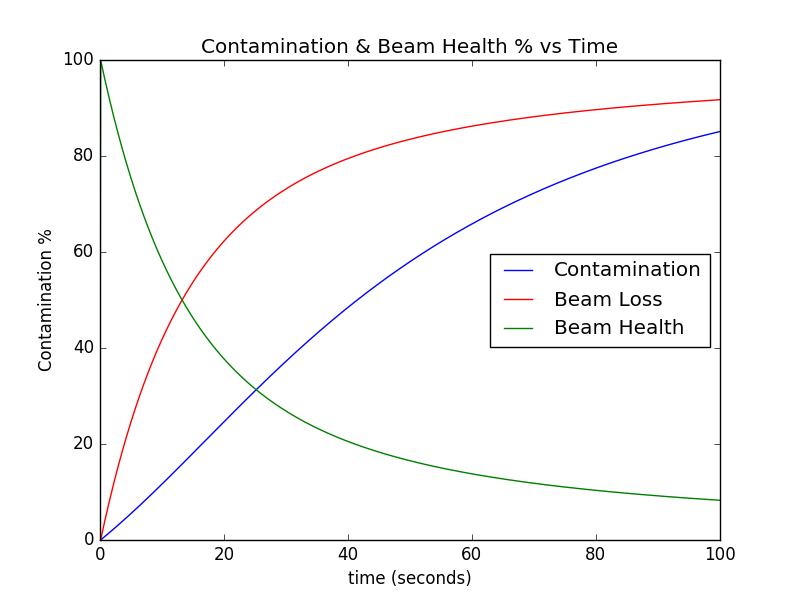
\includegraphics[width=0.5\linewidth]{./Images/Figures/figure_1-4}

A nicely formatted plot with a legend using the matplotlib package.
\begin{lstlisting}
import matplotlib as plt    # Imports the correct packages for plotting.

fig = plt.figure(dpi=1200)  # Increase resolution of the plot.
plt.scatter(x, y, s=0.1)    # Plot x data vs y data with a dot size of 0.1.
fig.suptitle(title, fontsize=12) # adds a title to the figure.

plt.xlabel("x axis label")  # Creates a x-axis label.
plt.ylabel("y axis label")  # Creates a y-axis label.

manage = plt.get_current_fig_manager()
manage.full_screen_toggle() # Makes the plt full screen.

plt.show()                  # Displays plot.
plt.savefig("fileName.png") # Saves the figure as an image
\end{lstlisting}





























\section{Pytest \index{Pytest}}

\idx{Pytest} is a powerful and popular testing framework for Python that simplifies the process of writing and executing tests. It offers a straightforward syntax and extensive features for writing test cases, including assertions, fixtures, parameterization, and test discovery. Pytest provides robust support for testing different types of applications, including web applications, APIs, and command-line utilities. It promotes efficient testing practices by emphasizing readability, scalability, and flexibility, making it a preferred choice for many Python developers.

\myindent To run a python test file using pytest, you can call pytest directly via a terminal.
\begin{lstlisting}
pytest -vv test_my_module.py
\end{lstlisting}

To write tests for a function, you must import that function and write a test for it. The \idx{assert} is a basic test keyword is used to check if a statement is true of false.
\begin{lstlisting}
# Code implementation in a Python file (e.g., my_module.py)

def add(x, y):
    """Function to add two numbers."""
    return x + y
\end{lstlisting}

\begin{lstlisting}
# Test case using Pytest (e.g., test_my_module.py)

import pytest
import my_module

def test_add():
    """Test case for the add function."""

    # Test with positive integers
    assert my_module.add(2, 3) == 5
    
    # Test with negative integers
    assert my_module.add(-2, -3) == -5
    
    # Test with zero
    assert my_module.add(0, 0) == 0
    
    # Test with one positive and one negative integer
    assert my_module.add(5, -3) == 2
\end{lstlisting}

A pytest \idx{fixture} can be used to create a \idx{temporary directory} for testing.

\begin{lstlisting}
import pytest

@pytest.fixture
def temp_directory():
    """
    Fixture to create a temporary directory for testing.

    This fixture creates a temporary directory using tempfile.mkdtemp().
    The temporary directory path is provided to the test functions, and after testing,
    the temporary directory is removed to clean up resources.

    Yields:
        str: Path of the temporary directory.
    """
    # Create a temporary directory for testing
    temp_dir = tempfile.mkdtemp()
    # Provide the temporary directory to the test for its duration.
    yield temp_dir

# Call a method using the temp_directory() method.
def test_method(temp_directory):
	print(temp_directory) # Prints the temp directory path
\end{lstlisting}

A pytest \idx{fixture} can be used to return an instance of a class.

\begin{lstlisting}
import pytest
from mmorpdnd import MMORPDND

@pytest.fixture
def mmorpdnd_instance():
    """
    Fixture to provide an instance of the MMORPDND class for testing.
    """
    return MMORPDND()
\end{lstlisting}

You can define a list of test \idx{parameters} to be input into a test via the \idx{@pytest.mark.parametrize} decorator, allowing multiple input-output pairs to be tested with the same test function.

\begin{lstlisting}
@pytest.mark.parametrize("input_string, expected_output", [
    ("'6 (barbarian 3, rogue 3)'", 6),
    ("'12 dwarfs and 3 elves'", 12),
    ("'No numbers here!'", None),
    ("'Only one number: 42'", 42),
    ("'Negative number: -10'", -10),
    ("'Integers: 1 2 3'", 1),
    ("'999'", 999),
])
def test_extract_first_integer(input_string, expected_output):
    """
    Test case to verify the behavior of extract_first_integer function.
    """
    assert extract_first_integer(input_string) == expected_output
\end{lstlisting}









\section{Python tk GUI}

Python \idx{Tkinter} (\idx{Tk}) is a built-in \idx{GUI} (Graphical User Interface) toolkit that allows developers to create desktop applications with a graphical interface in Python. Tkinter provides a set of widgets (such as buttons, labels, and entry boxes) and tools to arrange them within windows and frames. It is based on the Tk GUI toolkit originally developed for the Tcl programming language. With Tkinter, developers can create cross-platform applications that run on Windows, macOS, and Linux, making it a popular choice for simple to moderately complex desktop applications in Python. To install Tk on linux (APT), the following command can be used.

\begin{lstlisting}[style=terminalstyle]
sudo apt-get install python3-tk
\end{lstlisting}

A basic \idx{hello world} gui written in Tk follows:

\begin{lstlisting}
import tkinter as tk

def say_hello():
    label.config(text="Hello, World!")

# Create the main application window
gui = tk.Tk()
gui.title("Hello, Tkinter!")

# Create a label widget
label = tk.Label(gui, text="Click the button to say hello!")
label.pack(pady=10)

# Create a button widget
button = tk.Button(gui, text="Say Hello", command=say_hello)
button.pack()

# Run the Tkinter event loop
gui.mainloop()
\end{lstlisting}

To change the \idx{geometry} of a Tk gui window, the following can be used:

\begin{lstlisting}
gui = tk.Tk()
gui.geometry("300x470")
\end{lstlisting}

To change the \idx{icon} of a Tk gui window, the following can be used:

\begin{lstlisting}
# Load icon image
icon = PhotoImage(file=f'{root_dir}/img.png')
# Set icon image
gui.tk.call('wm', 'iconphoto', self.gui._w, icon)
\end{lstlisting}



























\section{Useful Methods and Packages}


\subsection{Useful Packages}

In this section, we explore Python's extensive collection of packages, offering tailored solutions for diverse tasks. Python's packages are specialized tools, empowering developers to address specific challenges efficiently. From data manipulation to machine learning, web development to scientific computing, Python packages provide a robust foundation for diverse projects.




\subsubsection{\idx{collections}}

Python's \idx{collections} module provides a \idx{Counter} class, which is a specialized dictionary designed for counting hashable objects. One lesser-known feature of Counter is that it supports arithmetic operations like \idx{addition}, \idx{subtraction}, \idx{intersection}, and \idx{union}. This is particularly useful when you're dealing with counting occurrences of items across different datasets or need to perform set-like operations on the counts themselves.
\begin{lstlisting}
from collections import Counter

# Define two Counters
counter1 = Counter({'a': 3, 'b': 1, 'c': 2})
counter2 = Counter({'a': 1, 'b': 2, 'd': 1})

# Addition: Adds counts from two counters
print("Addition:", counter1 + counter2)
# Prints "Addition: Counter({'a': 4, 'b': 3, 'c': 2, 'd': 1})"

# Subtraction: Subtracts counts, but keeps only positive results
print("Subtraction:", counter1 - counter2)
# Prints "Subtraction: Counter({'a': 2, 'c': 2})"

# Intersection: Keeps only positive counts common to both counters
print("Intersection:", counter1 & counter2)
# Prints "Intersection: Counter({'a': 1, 'b': 1})"

# Union: Keeps maximum counts from both counters
print("Union:", counter1 | counter2)
# Prints "Union: Counter({'a': 3, 'b': 2, 'c': 2, 'd': 1})"
\end{lstlisting}

Python's \idx{collections} module provides a class called \idx{defaultdict}, which is a subclass of the built-in dictionary (dict) class. The \idx{defaultdict} is similar to a regular dictionary, but it allows you to specify a default value factory for missing keys. This means that when you access a key that doesn't exist, instead of raising a \idx{KeyError}, defaultdict will create the key and assign it a default value returned by the factory function.
\begin{lstlisting}
from collections import defaultdict

# Create a defaultdict with int as the default value factory
d = defaultdict(int)

# Accessing a non-existent key will create it with a default value of 0
print(d['a'])  # Output: 0

# You can also specify a different default value factory
d = defaultdict(list)

# Accessing a non-existent key will create it with an empty list as the default value
print(d['b'])  # Output: []

# You can use any callable as the default value factory
d = defaultdict(lambda: 'default')

# Accessing a non-existent key will create it with 'default' as the default value
print(d['c'])  # Output: 'default'
\end{lstlisting}









\subsubsection{\idx{itertools}}

Python's \idx{itertools} module provides functions called \idx{combinations} and \idx{combinations\_with\_replacement}, which generates all possible \idx{combinations} of a given length from the elements of an \idx{iterable}, including combinations with repeated elements.
\begin{lstlisting}
from itertools import combinations

# Generate combinations of length 2 from the elements 'A', 'B', 'C' without replacement
combinations = combinations(['A', 'B', 'C'], 2)

# Print the generated combinations
for combo in combinations:
    print(combo, end=',')
# Prints "('A', 'B'),('A', 'C'),('B', 'C'),"
\end{lstlisting}
\begin{lstlisting}
from itertools import combinations_with_replacement

# Generate combinations of length 2 from the elements 'A', 'B', 'C' with replacement
combinations = combinations_with_replacement(['A', 'B', 'C'], 2)

# Print the generated combinations
for combo in combinations:
    print(combo, end=',')
# Prints "('A', 'A'),('A', 'B'),('A', 'C'),('B', 'B'),('B', 'C'),('C', 'C'),"
\end{lstlisting}











\subsubsection{\idx{slice}}

Python has a built-in \idx{slice} object that can be used to slice \idx{sequences} like \idx{lists}, \idx{tuples}, and \idx{strings}. While slicing with regular slicing syntax (list[start:end:step]) is common, creating and using slice objects directly can be powerful, especially when working with multiple slices or when you want to reuse the same slice configuration.
\begin{lstlisting}
# Create a slice object with start, stop, and step
my_slice = slice(1, 5, 2)

# Apply the slice to a list
my_list = ['a', 'b', 'c', 'd', 'e', 'f', 'g']
sliced_result = my_list[my_slice]

print(sliced_result)  # Output: ['b', 'd']

# You can also use the slice object with other sequences like strings
my_string = "Hello, World!"
sliced_string = my_string[my_slice]

print(sliced_string)  # Output: 'el'
\end{lstlisting}

In this example, slice(1, 8, 2) creates a \idx{slice} object that starts at index 1 ('b'), ends at index 8 ('i'), and steps by 2. So, applying this slice to the list ['a', 'b', 'c', 'd', 'e', 'f', 'g', 'h', 'i'], it selects elements at indices 1, 3, 5, and 7, which correspond to the values 'b', 'd', 'f', and 'h', respectively.
\begin{lstlisting}
# Create a slice object with start, stop, and step
my_slice = slice(1, 8, 2)

# Apply the slice to a list
my_list = ['a', 'b', 'c', 'd', 'e', 'f', 'g', 'h', 'i']
sliced_result = my_list[my_slice]

print(sliced_result)  # Output: ['b', 'd', 'f', 'h']
\end{lstlisting}












\subsubsection{\idx{functools}}

Python's \idx{functools} module provides a function called \idx{singledispatch}, which allows you to create a single-dispatch generic function. It allows you to define a function behavior based on the type of the first argument. This is particularly useful for creating functions that can handle different types of input in a flexible and extensible way, similar to \idx{method overloading} in other programming languages.
\begin{lstlisting}
from functools import singledispatch

@singledispatch
def my_func(arg):
    print("Default implementation:", arg)

@my_func.register(int)
def _(arg):
    print("Processing an integer:", arg)

@my_func.register(str)
def _(arg):
    print("Processing a string:", arg)

@my_func.register(list)
def _(arg):
    print("Processing a list:", arg)

# Test the function with different types of input
my_func(10)         # Output: Processing an integer: 10
my_func("Hello")    # Output: Processing a string: Hello
my_func([1, 2, 3])  # Output: Processing a list: [1, 2, 3]
\end{lstlisting}

Python's \idx{functools} module provides a decorator called \idx{lru\_cache}, which stands for "Least Recently Used Cache." It's a built-in memoization decorator that caches the results of a function and reuses them when the same inputs occur again. \idx{lru\_cache} Uses a least-recently-used (LRU) eviction policy. This means that when the cache reaches its maximum size (specified by the maxsize argument), the least recently used entries are discarded to make room for new ones.
\begin{lstlisting}
@lru_cache(maxsize=None)
def fib(n):
    if n < 2:
        return n
    return fib(n-1) + fib(n-2)

>>> [fib(n) for n in range(16)]
[0, 1, 1, 2, 3, 5, 8, 13, 21, 34, 55, 89, 144, 233, 377, 610]

>>> fib.cache_info()
CacheInfo(hits=28, misses=16, maxsize=None, currsize=16)
\end{lstlisting}

Python's \idx{functools} module provides a function called \idx{cache}, which allows you to cache the results of a function call and reuse them when the same inputs occur again. This can significantly improve the performance of your code, especially when dealing with expensive computations or I/O operations. This was introduced in python 3.9. Unlike \idx{lru\_cache}, \idx{cache} Does not have a built-in eviction policy. It simply caches results until the program exits or until the function is explicitly uncached. Because it never needs to evict old values, this is smaller and faster than \idx{lru\_cache} with a size limit.

\begin{lstlisting}
from functools import cache

@cache
def factorial(n):
    return n * factorial(n-1) if n else 1

>>> factorial(10)      # no previously cached result, makes 11 recursive calls
3628800
>>> factorial(5)       # just looks up cached value result
120
>>> factorial(12)      # makes two new recursive calls, the other 10 are cached
479001600
\end{lstlisting}





\subsubsection{\idx{typing}}

Python's \idx{typing} module provides a way to specify type hints for variables, function arguments, and return values. While type hints are often used for improving code readability and catching errors early during development, you can also use them for \idx{runtime} type checking using the typing module's \idx{runtime\_checkable} decorator along with the \idx{Protocol} class. In this example, Printable is defined as a protocol using the Protocol class. It specifies a method print that takes no arguments and returns None. By decorating Printable with @runtime\_checkable, you enable runtime type checking for objects that claim to conform to the protocol. The print\_if\_possible function takes an argument of type Printable and calls its print method. When called with an object that conforms to the Printable protocol (like Printer), it works fine. However, if called with an object that does not conform to the Printable protocol (like NotPrinter), it raises a TypeError, allowing you to catch potential type errors at runtime.
\begin{lstlisting}
from typing import Protocol, runtime_checkable

# Define a protocol with type hints for methods
@runtime_checkable
class Printable(Protocol):
    def print(self) -> None:
        pass

# A class that conforms to the Printable protocol
class Printer:
    def print(self) -> None:
        print("Printing...")

# A class that does not conform to the Printable protocol
class NotPrinter:
    def display(self) -> None:
        print("Displaying...")

def print_if_possible(obj: Printable) -> None:
    obj.print()

printer = Printer()
not_printer = NotPrinter()

# This will work fine since Printer conforms to the Printable protocol
print_if_possible(printer)

# This will raise a TypeError since NotPrinter does not conform to the Printable protocol
print_if_possible(not_printer)
\end{lstlisting}







\subsubsection{\idx{enum}}

Python's \idx{enum} module provides a powerful way to create \idx{enumerations} in Python. Enumerations allow you to define symbolic names (members) for a set of unique values, which can make your code more readable and maintainable. One lesser-known feature of enumerations is the ability to create them dynamically using the Enum class's functional API. This allows you to create enumerations without explicitly subclassing Enum.
\begin{lstlisting}
from enum import Enum

# Define a dynamic enumeration
DynamicEnum = Enum("DynamicEnum", ["VALUE1", "VALUE2", "VALUE3"])

# Access enumeration members
print(DynamicEnum.VALUE1)  # Output: DynamicEnum.VALUE1
print(DynamicEnum.VALUE2)  # Output: DynamicEnum.VALUE2
print(DynamicEnum.VALUE3)  # Output: DynamicEnum.VALUE3
\end{lstlisting}


To access an \idx{enum} name from an \idx{enum} class based on an the value, you can write a method to access the enum values and compare to another value.
\begin{lstlisting}
from enum import Enum

class Color(Enum):
    RED = 1
    GREEN = 2
    BLUE = 3

def get_enum_from_value(value):
    for color in Color:
        if color.value == value:
            return color
    raise ValueError("No enum member with that value")

color = get_enum_from_value(2)
print(color)  # Output: Color.GREEN
\end{lstlisting}






\subsubsection{\idx{contextlib}}

Python's \idx{contextlib} module provides a decorator called \idx{contextmanager}, which allows you to create context managers using generator functions. Context managers are objects that define \_\_enter\_\_ and \_\_exit\_\_ methods, and they are commonly used with the with statement to manage resources, such as opening and closing files or acquiring and releasing locks.
\begin{lstlisting}
from contextlib import contextmanager

@contextmanager
def open_file(filename, mode):
    file = open(filename, mode)
    try:
        yield file
    finally:
        file.close()

# Usage of the context manager
with open_file("example.txt", "w") as f:
    f.write("Hello, context managers!")
\end{lstlisting}

Python's \idx{contextlib} module provides utilities for working with context managers. One lesser-known feature of the \idx{contextlib} module is the \idx{redirect\_stdout} and \idx{redirect\_stderr} context managers, which allow you to temporarily redirect the standard output and standard error streams to a specified file or file-like object.
\begin{lstlisting}
from contextlib import redirect_stdout
import io

# Create a StringIO object to redirect output
output_buffer = io.StringIO()

# Redirect stdout to the StringIO object
with redirect_stdout(output_buffer):
    print("This will be captured by the redirect_stdout context manager")

# Get the captured output from the StringIO object
captured_output = output_buffer.getvalue()

print("Captured Output:", captured_output)
# Prints "Captured Output: This will be captured by the redirect_stdout context manager"
\end{lstlisting}


























\subsection{Useful Methods}

Thsi section is a collection of useful methods that can be adapted or used for many applications. These are all methods that I've written or heavily modified for my own use and have found useful on multiple occasions.

\subsubsection{Logging and Application Output}

To perform \idx{logging} for an application, you often want to create a \idx{log file} named based on the application name and the current date. This can be expanded to be contained in a class and called during initialization or just used as standalone.

\begin{lstlisting}
#!/bin/python3
import os
import sys

# Used for gathering time and date data.
from datetime import datetime


def set_log_file_name():
    """
    Returns the log file name. If it has not yet been set, creates the log filename that contains the date and then returns it.
    
    The desired behavior is that one log_file is used per run of the application. 
	To account for day changes while the program is running, log_file must be created at application runtime.
    """    
    global log_file
    
    # Get the script name with full path
    script_path = os.path.abspath(sys.argv[0])
    # Get the script name without the extension.
    script_name = os.path.basename(script_path).split('.py')[0]
    
    # Check if the log file already has been set.
    if log_file == "":
        today = datetime.today().strftime("%Y%m%d")
        log_file = f"{script_name}_log_{today}"
        
    return log_file

# The log file to be used throughout the file.
log_file = ""
set_log_file_name()
\end{lstlisting}

With a \idx{log file} defined, you can perform \idx{logging} by appending messages to a log file. The message can include a \idx{time stamp} for referencing when various tasks were performed at a later date.

\begin{lstlisting}
# Used for gathering time and date data.
from datetime import datetime


def log_text(text, include_time_stamp=True):
    """
    This will output text to the logfile with an optional time stamp.
    Args:        
        text (str): The text to be logged.
        timestamp (bool): Option to include timestamp in logging.    
    """
    # Set's the appropriate timestamp value to use.
    if include_time_stamp:
        timestamp_text = datetime.now().strftime("[%Y-%m-%d %H %M %S]")
    else:
        timestamp_text = ""

    # Logs the output. This assumes log_file is defined.
    with open(log_file, 'a') as log:            
        log.write(f"{timestamp_text} {text}\n")
\end{lstlisting}

When writing an application with complex or varied output, it is often useful to \idx{print} messages to the terminal using various \idx{color codes}. To do this, you can write a method that takes either various types of options (each corresponding to a color code) or takes a color name directly. You can also modify it to optionally automatically log the information using the log\_text() method defined above. This is a highly adaptable code snippet.

\begin{lstlisting}
def output_text(text:str, option:str=None , color:str=None , log=True):
    """
    Print text in different colors based on the provided option. This will also log the output text (including a time stamp).

    Args:
        text (str): The text to be printed and logged.
        option (str): The color option for the text. Valid options are defined in the color mappings list (second element). Default = None.
        color (str): The color name for the text. Valid options are defined in the color mappings list (first element). Default = None.
        log (bool): Determines whether to log the text or not. Default = True.        

    Returns:
        None

    Note:
        This function uses ANSI escape codes for color formatting. Colors may not be displayed correctly in all environments. The color and option parameters should not both be used. If they are, the color will override the option parameter.
    """
    # Defines the default behaviour.
    if color == None and option == None:
        color = "white"  
    if color != None and option != None:
        option = None
    if color == None:
        color = ""
    if option == None:
        option = ""
        
    # Define the list of color mappings
    color_mappings = [
        ("white",   "text",    "\033[0m"),      # White/default/reset
        ("red",     "error",   "\033[91m"),     # Red
        ("green",   "success", "\033[92m"),     # Green
        ("yellow",  "warning", "\033[93m"),     # Yellow
        ("blue",    "note",    "\033[94m"),     # Blue
    ]
    
    # Set's the reset value for normal text.
    reset_code = "\033[0m"
    found_match = False    
    
    for color_name, color_type, color_code in color_mappings:
        if color.lower() == color_name:
            print(f"{color_code}{text}{reset_code}")
            found_match = True
            break
        elif option.lower()  == color_type:
            print(f"{color_code}{text}{reset_code}")
            found_match = True
            break
            
    # If no color match was found, print the text.         
    if not found_match:
            print(text)
    
    if log:
        log_text(text)
\end{lstlisting}

\begin{fancybox}[ANSI Color Codes For Terminal Output]{1}
The American National Standards Institute (\idx{ANSI}) \idx{color codes} in the above can be expanded further if the application needs more color outputs. The below chart can be used.
	\begin{longtable}{|l|l|l|}
	\hline
	\textbf{Color Name} & \textbf{ANSI Escape Code} & \textbf{Example} \\
	\hline
	White & \texttt{\textbackslash 033[0m} & \textcolor{white}{Text} \\
	\hline
	Black & \texttt{\textbackslash 033[30m} & \textcolor{black}{Text} \\
	\hline
	Red & \texttt{\textbackslash 033[91m} & \textcolor{red}{Text} \\
	\hline
	Green & \texttt{\textbackslash 033[92m} & \textcolor{green}{Text} \\
	\hline
	Yellow & \texttt{\textbackslash 033[93m} & \textcolor{yellow}{Text} \\
	\hline
	Blue & \texttt{\textbackslash 033[94m} & \textcolor{blue}{Text} \\
	\hline
	Magenta & \texttt{\textbackslash 033[35m} & \textcolor{magenta}{Text} \\
	\hline
	Cyan & \texttt{\textbackslash 033[36m} & \textcolor{cyan}{Text} \\
	\hline
	Gray & \texttt{\textbackslash 033[90m} & \textcolor{gray}{Text} \\
	\hline
	Purple & \texttt{\textbackslash 033[95m} & \textcolor{purple}{Text} \\
	\hline
	Orange & \texttt{\textbackslash 033[33m} & \textcolor{orange}{Text} \\
	\hline
	\end{longtable}
\end{fancybox}










\unchapter{Resources}


%Begin the backmatter.
\backmatter
{\footnotesize
\begin{thebibliography}{99}
	\bibitem{cpp:pointers} http://www.cplusplus.com/doc/tutorial/pointers/
	
	\bibitem{cpp:chrono} http://www.cplusplus.com/reference/chrono/
	
	\bibitem{linux:networking commands} Kumar, Chandan. “10 Useful Linux Networking Commands.” Geek Flare, 11 Feb. 2018, geekflare.com/linux-networking-commands/. 
	
	\bibitem{linux: shell scripting}  Parker, Steve. “Shell Scripting Tutorial.” The Shell Scripting Tutorial, www.shellscript.sh/. 
\end{thebibliography}
}

\printindex

\end{document}